\documentclass[10pt]{article}
\usepackage[margin=0.75in]{geometry}
\usepackage{graphicx,booktabs,float,caption,hyperref,microtype,amsmath}
\usepackage[T1]{fontenc}
\usepackage{lmodern}
\hypersetup{hidelinks}
\setlength{\parskip}{4pt}\setlength{\parindent}{0pt}
\title{\textbf{COP5612 Project 3: Pastry Overlay and Key/Value Service in Erlang}}
\author{Surya Charan Perisetla}
\date{Fall 2026}
\begin{document}\maketitle

\section{Objective}
This project implements the Pastry protocol of Rowstron and Druschel (network join and routing) in Erlang using the actor model.
On top of it runs a simple object access service that associates a key, drawn from the same id space as the node ids, with a string.
Every peer is one Erlang process, and all interaction between peers is asynchronous message passing.
The program is started as \texttt{project3 numNodes numRequests}.
It builds a network of \texttt{numNodes} peers, then every peer makes \texttt{numRequests} requests at one request per second.
When all peers have finished, the program prints the average number of hops (node to node connections) that a message traversed to be delivered.

\section{Design}
\subsection{Actors}
\begin{itemize}
  \item \textbf{Peer} (\texttt{pastry\_node}): one actor per peer. It holds the Pastry state, runs the join and routing protocols, and hosts the application.
  \item \textbf{Collector} (\texttt{pastry\_collector}): receives one report per finished request, accumulates the hop statistics, and checks every answer against the true ring.
  \item \textbf{Main} (\texttt{project3}): creates the peers, joins them, seeds the store, starts the request phase and prints the result.
\end{itemize}

\subsection{Identifiers and node state}
Node ids and keys are 128-bit integers on a circular id space (MD5 is used in place of SHA-1).
With $b = 4$ an id is read as 32 hexadecimal digits.
Each peer keeps the three tables from Section 2.1 of the paper:
\begin{itemize}
  \item \textbf{Routing table} $R$: 32 rows of 16 columns. Row $l$ holds nodes that share the first $l$ digits with the present node and differ in digit $l$; the column is the value of that digit.
  \item \textbf{Leaf set} $L$ ($|L| = 16$): the 8 numerically closest smaller ids and the 8 numerically closest larger ids on the ring.
  \item \textbf{Neighborhood set} $M$ ($|M| = 16$): the 16 nodes closest to the present node by the proximity metric.
\end{itemize}
Every peer is given random coordinates in a $1000 \times 1000$ plane, and the euclidean distance between two peers serves as the proximity metric.
When two candidates qualify for the same routing table slot, the closer one is kept.
This gives Pastry's locality property: routing table entries point to nearby nodes.

\subsection{Routing}
Routing follows Table 1 of the paper.
When a message with key $D$ arrives at node $A$:
\begin{enumerate}
  \item If $D$ lies within the range of the leaf set, the message goes to the leaf whose id is numerically closest to $D$, or is delivered at $A$ if $A$ itself is closest.
  \item Otherwise, let $l$ be the length of the prefix shared by $D$ and $A$. If the routing table entry $R[l][D_l]$ exists, the message goes there.
  \item Otherwise (the rare case), the message goes to any node known to $A$ (in $L$, $R$ or $M$) that shares a prefix of at least $l$ digits with $D$ and is numerically closer to $D$ than $A$.
\end{enumerate}
Each step either lengthens the shared prefix or brings the message numerically closer to the key, so a message cannot loop.
The hop counter is incremented each time a message is passed from one node to another.

\subsection{Network join}
Nodes join one at a time, following Section 2.4 of the paper.
\begin{enumerate}
  \item The new node $X$ is given a node $A$ that is close to it by the proximity metric (the nearest of a random sample of already joined nodes).
  \item $X$ asks $A$ to route a special \emph{join} message with key equal to $X$'s id.
  \item Every node on the path, from $A$ to the node $Z$ whose id is numerically closest to $X$, sends its state tables to $X$.
  \item $X$ builds its routing table from these tables, takes its leaf set from $Z$ and its neighbours, and takes its neighborhood set from the nodes that are closest by proximity.
  \item $X$ sends its state to every node in its tables. Those nodes update their own tables and acknowledge. When all acknowledgements have arrived, the join is complete.
\end{enumerate}
The \texttt{--verify} option compares every node's leaf set with the true ring neighbours after the join phase.
At every size tested (10 to 20\,000 nodes, 3 runs each), 100\% of the leaf sets matched.

\subsection{Pastry API}
The interface follows Section 2.3 of the paper.
\begin{itemize}
  \item \texttt{pastry\_node:start/5} corresponds to \texttt{pastryInit(Credentials, Application)}: it creates a node with its id and coordinates, bound to an application module, and returns the node id.
  \item \texttt{pastry\_node:route/3} corresponds to \texttt{route(msg, key)}.
  \item The application module implements the upcalls \texttt{deliver(msg, key)}, called on the node responsible for the key; \texttt{forward(msg, key, nextId)}, called on each intermediate node before forwarding; and \texttt{newLeafs(leafSet)}, called whenever the leaf set changes.
\end{itemize}

\subsection{Object access service}
The application (\texttt{kv\_app}) stores strings under keys.
\begin{itemize}
  \item \texttt{put(key, string)} is routed to the root of the key (the node numerically closest to it), which stores the string and copies it to its 2 closest leaves.
  \item \texttt{get(key)} is routed the same way, and the root sends the string straight back to the requester.
\end{itemize}
Before the request phase, $\min(N, 10\,000)$ objects (at least 16) are stored with \texttt{put}.
Each request is then, with equal probability, a \texttt{get} of a random stored object or a \texttt{put} of a new string.
For every \texttt{get}, the requester checks that the returned string is exactly the one that was stored.
Every peer issues one request per second, and the first request of each peer is offset by a random fraction of a second so that requests do not all start at once.

\subsection{Correctness check}
The collector knows every node id.
For every answered request, it checks that the answering node really is the node numerically closest to the key.
In every run without failures, 100\% of requests passed this check and every \texttt{get} returned the right string.

\section{Experiments}
Each network size was run 3 times with different random seeds, with 10 requests per peer.
The machine was a 14 core laptop with 24\,GB of RAM.

\begin{table}[H]
\centering\small
\caption{Average hops per request (mean of 3 runs, 10 requests per peer). The two largest networks were run once, with 3 and 2 requests per peer.}
\begin{tabular}{@{}r rrr r r@{}}
\toprule
\textbf{Nodes $N$} & \textbf{Requests} & \textbf{Avg hops} & $\log_{16} N$ & \textbf{Routed correctly} & \textbf{Join time}\\
\midrule
10      & 100       & 0.91 & 0.83 & 100\% & 0.01 s\\
50      & 500       & 1.44 & 1.41 & 100\% & 0.02 s\\
100     & 1\,000    & 1.70 & 1.66 & 100\% & 0.03 s\\
500     & 5\,000    & 2.21 & 2.24 & 100\% & 0.13 s\\
1\,000  & 10\,000   & 2.48 & 2.49 & 100\% & 0.30 s\\
2\,000  & 20\,000   & 2.70 & 2.74 & 100\% & 0.68 s\\
5\,000  & 50\,000   & 2.96 & 3.07 & 100\% & 1.98 s\\
10\,000 & 100\,000  & 3.24 & 3.32 & 100\% & 4.42 s\\
20\,000 & 200\,000  & 3.50 & 3.57 & 100\% & 10.0 s\\
100\,000 & 300\,000 & 3.99 & 4.15 & 100\% & 101 s\\
200\,000 & 400\,000 & 4.27 & 4.40 & 100\% & 609 s\\
\bottomrule
\end{tabular}
\end{table}

\begin{figure}[H]
\centering
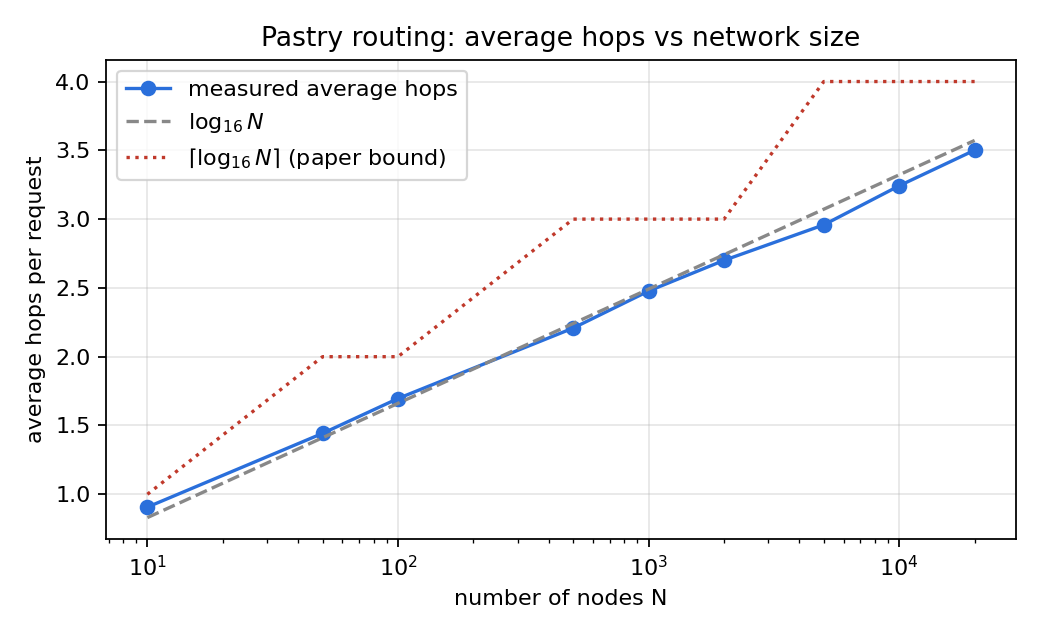
\includegraphics[width=0.75\linewidth]{hops_vs_nodes.png}
\caption{Average hops per request against network size (3 runs per size, 10 to 20\,000 nodes).}
\end{figure}

\textbf{Distribution of hops.} For a single run with 5\,000 nodes and 5 requests per peer (25\,000 requests), the hop counts were:
0 hops: 10, 1 hop: 278, 2 hops: 3\,746, 3 hops: 17\,660, 4 hops: 3\,293, 5 hops: 13.
So 99.95\% of messages were delivered within $\lceil \log_{16} 5000 \rceil = 4$ hops.

\section{Discussion}
\begin{itemize}
  \item \textbf{Hop count grows logarithmically.} The average number of hops follows $\log_{16} N$ closely, from 0.91 hops at 10 nodes to 4.27 hops at 200\,000 nodes, and stays just below it for larger networks.
  This matches the paper's claim that Pastry delivers a message in fewer than $\lceil \log_{2^b} N \rceil$ steps on average.
  Each hop fixes one more digit of the key with the routing table, and the leaf set completes the last step.
  \item \textbf{Small networks.} At 10 and 50 nodes the average is slightly above $\log_{16} N$, because the whole network fits in the leaf set, so almost every message takes exactly one hop.
  Only the few requests whose requester is itself the root take zero hops.
  \item \textbf{Routing is always correct.} Every request in every run reached the node numerically closest to its key, and every \texttt{get} returned the stored string.
  \item \textbf{Scaling limits.} The join phase is sequential, and each join costs $O(\log N)$ routing hops plus messages to the roughly 100 nodes in the new node's tables.
  Join time grows somewhat faster than linearly at the largest sizes, mostly because of memory pressure.
  At 100\,000 nodes and more, the laptop cannot sustain one request per second per peer (over 100\,000 routed messages per second plus replication), so requests queue up and the request phase takes longer than \texttt{numRequests} seconds. All requests still complete.
\end{itemize}

\section{Largest network}
The largest network run was \textbf{200\,000 nodes} (\texttt{./project3 200000 2}).
All 400\,000 requests were answered correctly by the correct root, with an average of 4.27 hops.
The join phase took about 10 minutes and the memory use was 10.4\,GB (max resident set size).
Memory is the limit beyond this size, since each actor keeps about 100 node descriptors.

\section{Bonus}
The failure models (node crashes, and temporary and permanent link failures), the mechanisms that handle them, and the experiments are described in the separate report \texttt{Report-bonus.pdf}.
\end{document}
